\section{Modèle d'exécution fluxionnel}

\subsection{Fluxions}

Le principe du modèle d'exécution fluxionnel est d'identifier des unités d'exécution autonomes n'ayant pour paramètre d'entrée et de sortie que des flux, c'est à dire des séquences continues et infinies de données agrégés par messages.
Nous avons appelé cette unité d'exécution autonome une fluxion.
C'est à dire une fonction, au sens de la programmation fonctionnelle, dépendant exclusivement de flux de données.
Elle est composée d'un nom unique, d'une fonction de traitement, et d'un contexte mémoire au moment de son exécution.

Les entrées et sorties d'une fluxion sont des flux.
Un flux est un ensemble de messages à destination d'une fluxion.
Les messages sont composés du nom de la fluxion destinataire et d'un corps.
Ils représentent à la fois le signal d'invocation, et les données nécessaires à cette invocation.
Après avoir traité un message, la fonction de traitement modifie son contexte local, puis se termine en renvoyant un message sur son flux de sortie.
% La fonction de traitement sait à quelles fluxions les messages de sortie doivent être délivré.
% Toute la logique d'une application fluxionnel se trouve dans les fluxions, il n'est pas masqué par une interface de messagerie et un système de routage.

Les fluxions forment des chaînes de traitement lié par les flux, transporté par un système de messagerie d'écrit plus bas.
% À la réception d'un message de démarrage, la fluxion destinataire va envoyer un second message à une autre fluxion, qui elle même va renvoyer un troisième message à une fluxion différente, et ainsi de suite.
Les fluxions sont organisés dans un graph dirigé. (note: le graphe n'est pas acyclique)
Chaque fluxion renvoie un message unique à destination d'une ou plusieurs fluxions.

Le contexte d'exécution de la fonction de traitement est l'ensemble des variables de mémoire dont dépend la fluxion pour poursuivre un traitement entre deux exécutions.
% En dehors du contexte d'exécution, la fonction de traitement ne peut pas persister de mémoire d'une exécution à l'autre.

% \TODO{	
% Les données et la logique d'une application étant cloisonné de manière distincte pendant l'exécution, il est possible de mettre à jour une fluxion en la remplaçant dans le système, sans impacter l'exécution de l'application.
% }

% Une fluxion peut être déplacée dynamiquement d'environnement d'exécution au cours de son activité.
% Déplacer une fluxion nécessite de déplacer sa fonction de traitement ainsi que son contexte d'exécution.
% Dans notre approche, nous avons distingué et cloisonné le contexte d'exécution, les paramètres d'appel et les paramètres de retour dans des flux.
% Mesurer le débit de ces flux permet d'estimer le coup de leurs déplacements.
% Ainsi, déplacer une fluxion consiste à déplacer le code fonctionnel vers une nouvelle destination, puis à rediriger ses flux d'entrées, de sorties et son contexte d'exécution en conséquence.



\subsection{Système de messagerie}

Le système de messagerie permet d'acheminer les flux entre les fluxions selon leurs noms.
% Toute l'exécution est orchestré par ce système de messagerie.

% Lorsqu'un message ou un groupe de message est soumis à l'envoie, soit par l'appel à \texttt{start}, soit au retour d'une fluxion, le système de messagerie le prend en charge.

% TODO à reformuler
% Pour chaque message, le système vérifie que la fluxion destinataire existe.
% Il appel la fonction de traitement de la fluxion destinataire, en utilisant son contexte d'exécution, et avec pour paramètre le corps du message.
% La fonction de traitement retourne un message, à son tour soumis à l'envoie.

Les messages soumis à l'envoi sont poussés dans une file, en attendant d'être traité par le système de messagerie.

\begin{algorithm}
\caption{Algorithme de traitement de la file de messages}
\begin{algorithmic}
\Function{ProcessMsg}{$msg$}
\For{$dest$ \textbf{in} $msg.dest$}
\State $flx \gets lookup(dest)$
\State $res \gets$ \Call{exec}{$flx, msg.body$}
\State \Call{enqueue}{$res$}
\EndFor
\EndFunction
\end{algorithmic}
\end{algorithm}

\begin{algorithm}
\caption{Algorithme de parcours de la file}
\begin{algorithmic}
\Function{ProcessMsg}{$msg$}
\While{$msg$ \textbf{presents in} $msgQueue$}
\State $msg \gets$ \Call{dequeue}{\null}
\State \Call{ProcessMsg}{$msg$}
\EndWhile
\EndFunction
\end{algorithmic}
\end{algorithm}

La fonction de traitement ne sera appelé qu'avec un seul paramètre : le message reçu.
% Ce message peut être vide, auquel cas, ce paramètre sera indéfini.

La fonction de traitement doit renvoyer un message, ou un tableau de plusieurs messages.
Un message se compose du nom de la fluxion destinataire, et optionnellement d'un corps.
Il se construit sous la forme suivante :

\begin{code}
{
  dest: "ma_fluxion", // nom de la fluxion destinataire du message
  body: // corps du message, optionnel
      {}, [], "", ...
}
\end{code}

\begin{figure}[h!]
  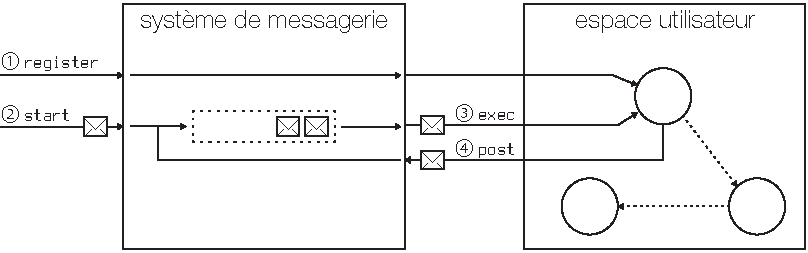
\includegraphics[width=0.5\textwidth]{schema-message.pdf}
  \caption{Schema du système de messagerie}
  \label{fig:messagerie}
\end{figure}

Pour exécuter un programme exprimé sous la forme de fluxions, le modèle d'exécution fluxionnel propose deux fonctions d'interface : l'enregistrement et le démarrage.
Le schema \ref{fig:messagerie} présente les différente étape dans l'acheminement d'un message.

Lors de l'initialisation du programme, il est nécessaire d'enregistrer les fluxions pour qu'elles puissent ensuite recevoir des messages.L'enregistrement se fait à l'aide de la fonction \texttt{register(<nom>, <fn>, <contexte>)}.
Le nom de la fluxion lui permet d'être identifié de manière unique dans le modèle d'exécution, et ainsi de recevoir des messages.
Il ne peut donc pas exister plusieurs fluxions ayant le même nom.
Une fluxion peut elle-même enregistrer d'autres fluxions dynamiquement.

% L'exécution d'une fluxion n'est déclenchée que par la réception d'un message.
L'exécution des fluxions enregistré dans le modèle d'exécution se fait en envoyant un message à une première fluxion, qui va elle même envoyer un message à une seconde et ainsi de suite.
% L'exécution d'une fluxion est déclenchée par le système de messagerie qui traite tous les messages en attente.
Pour déclencher cette chaîne un premier message est envoyé au système de messagerie en utilisant la fonction \texttt{start(<nom>,<msg>)}, étape \circled{2} sur le schema \ref{fig:messagerie}.
Cette fonction va placer un premier message dans la file du système de messagerie.
Le système exécute la fonction de traitement destinataire de ce premier message, étape \circled{3} sur le schema \ref{fig:messagerie}.
Le message résultat de cette exécution est alors empilé dans la file de message, étape \circled{4} sur le schema \ref{fig:messagerie}.

L'empilement des messages dans une file permet d'exécuter en parallèle plusieurs chaîne de traitement indépendantes de manière équitable.
Pour des raisons de performance, il pourrait être intéressant de lier les fluxions présentes sur le même nœud les unes derrières les autres, cependant, cela empêcherais les messages provenant du réseau d'être traité de manière équitable.

\subsection{Interface}

Le système fluxionnel ne manipule que des fluxion par l'intermédiaire d'un système de messagerie.
Afin de pouvoir interagir avec le monde extérieur, il faut définir des interfaces de bordure.
Les bordures du systèmes sont des fluxions qui font l'interface avec l'extérieur du système.

Notre approche repose sur une espérance de gain technologique principalement sur les architectures Web.
Le premier point d'entré visé est l'intégration des interfaces REST, mais tout autre point d'entrée est valable tant qu'une interface de bordure en flux peut être défini.

Dans notre approche, il existe deux types de fluxion de bordures web :

\begin{itemize}
	\item[les \textbf{entrées}]
    permettent de recevoir des connections client entrantes suivant le protocole HTTP.
    C'est donc le premier maillon de la chaîne de traitement.
    Pour chaque connexion entrante, l'entrée va générer une bordure de sortie permettant de répondre au client.
	\item[les \textbf{sorties}]
    permettent d'envoyer le résultat de la chaîne de traitement au client.
    C'est donc le dernier maillon de la chaîne de traitement.
\end{itemize}


Le schéma \ref{fig:schemaweb} présente les éléments d'un système Web fluxionnel et détaille les étapes d'acheminement d'un message par le système de messagerie.

\begin{figure}[h!]
	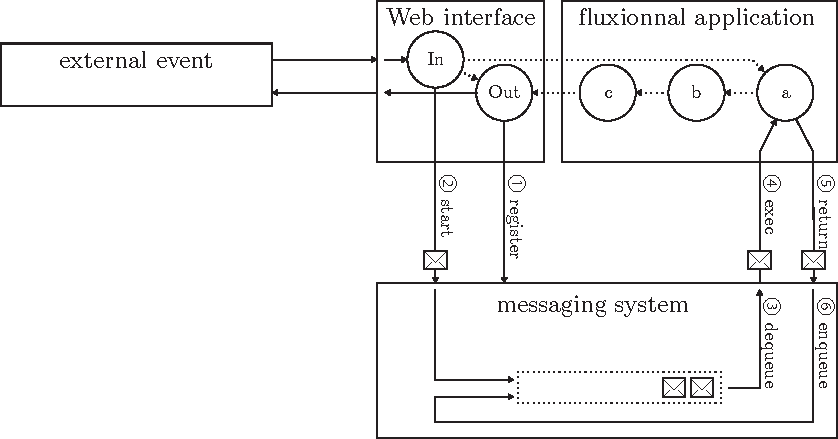
\includegraphics[width=0.5\textwidth]{schema-web.pdf}
	\caption{Schema d'un système fluxionnel avec une interface web}
	\label{fig:schemaweb}
\end{figure}

Le système Web est donc le déclencheur d'une chaîne de traitement de requêtes à chaque nouvelle requête d'un utilisateur un appel à la fonction \lstinline|start('/', <param>)| est réalisé dans le système de messagerie.
Au démarrage du système Web, deux fluxions de bordure sont lancées.
La fluxion de bordure 'in' n'est pas enregistré dans le système de messagerie.
Elle prend les paramètres de la requête Web, place l'identifiant de la connexion client dans le contexte de la demi-fluxion de sortie, puis lance le traitement de la requête en invoquant la fonction `start` du système de messagerie.

\subsection{Exemple de fluxion}

Afin d'illustrer le modèle d'exécution fluxionnel, nous présentons ici un exemple de son utilisation à travers un simple service de comptage de visite.

Ce service permet de compter le nombre de connexions HTTP de chaque utilisateur sur ce service et renvoie le résultat sous forme d'une réponse HTTP.

Le code \ref{lst:classique} représente le code de ce service de comptage dans un modèle classique.

\begin{figure}
  \begin{code}
  var app = require('express')();

  var count = {};

  app.get('/:id', function(req, res){
    res.send(req.params.id + '[' + (count[req.params.id] = (count[req.params.id] + 1) || 1 ) + ']');
  });

  port = 8080;
  app.listen(port);
  console.log("Listening port: "+port);
  \end{code}
  \caption{Code classique}
  \label{lst:classique}
\end{figure}

Le code \ref{lst:fluxionnel} représente le code de ce même service de comptage dans le modèle fluxionnel.

\begin{figure}
  \begin{code}
  var flx = require('./lib/flx')
    , express = require('express')
    , app = express();

  flx.register("output", function(msg){
    if (msg.res) {
      this.cid[msg.cid] = msg.res;
    } else {
      this.cid[msg.cid].send(msg.view.toString());
    }
    return undefined;
  }, {
    cid: {}
  })

  flx.register("input", function(msg){
    this.uid[msg.uid] = this.uid[msg.uid] + 1 || 1;
    msg.count = this.uid[msg.uid];
    return this.m("view", msg);
  },{
    uid: {}
  });

  flx.register("view", function(msg) {
    msg.view = msg.uid + "[" + msg.count + "]";
    msg.uid = undefined;
    msg.count = undefined;
    return this.m("output", msg);
  })

  app.get('/:id', function(req, res) {
    var uid = req.params.id;
    var cid = req.client._idleStart;

    flx.start(flx.m("output", {cid: cid, res: res}));
    flx.start(flx.m("input", {uid: uid, cid: cid}));
  })

  app.listen(8080);
  \end{code}
  \caption{Code fluxionnel}
  \label{lst:fluxionnel}
\end{figure}

La code classique est bien plus concis que le code fluxionnel du fait de la segmentation et de l'encapsulation  par le modèle fluxionnel.

Le service à été ségmenté comme suit :
\begin{itemize}
  \item Le point d'entrée \texttt{app.get} réagit à la connection d'un client et démarre la chaîne de traitement.
  Ce n'est pas une fluxion et il n'est pas enregistré dans le système de messagerie.
  \item Le point de sortie \texttt{output} est une fluxion mais elle est liée à la machine sur laquelle arrive la connexion afin de pouvoir y répondre.
  \item La fluxion \texttt{input} est la première à recevoir le message indiquant une connexion cliente. Son traitement consiste à incrémenter le compteur de l'utilisateur présent dans son scope, et à renseigner ce compteur dans le message, avant de le renvoyer à la fluxion suivante.
  \item La fluxion \texttt{view} récupère le message, et met en forme la réponse que recevra l'utilisateur, et l'envoie à la fluxion de sortie.
\end{itemize}

Les messages échangés contiennent principalement deux informations importantes : les identifiants d'utilisateurs, permettant d'incrémenter un compteur pour chaque utilisateur, et les identifiants de connexion, permettant de lier une suite de messages avec la structure contenant la connexion HTTP.
Le point d'entrée, et le point de sortie du système doivent rester sur la machine où la connexion a eu lieu pour avoir accès à l'interface réseau, tandis que les autre fluxions n'ont pas cette obligation, et peuvent être migré.


Cet identifiant de connexion est nécessaire au point de sortie pour associer le résultat reçu avec la connexion vers laquelle le renvoyer à l'utilisateur.
Nous passons cet identifiant pour ne pas alourdir les échanges de messages avec la structure contenant la connexion HTTP.

Ainsi, la fluxion de sortie reçois des messages provenant de deux fluxions : le point d'entrée




